As we already know a FRS takes a face as an input image, propagates it throw a NN and as a result returns probability distribution over set of personalities. When we talk about attack on FRS we mean we want either face A be recognized as face B (it is called Impersonation) or to face be A be recognized as any face but A (it is called Dodging). In the paper authors have focused on so-called adversarial attacks. In such attack assailant attacks an input of face recognition system by adding some (imperceptible to man) noise to this input (See Figure 12). Then this affected input (image) is transferred to the biometric system and incorrectly recognized.
 

\subsection{Impersonation}

In impersonation attack, an attacker seeks to be recognized as a specific different, exact user from FRS database. E.g. the adversary wants to log into another user android phone which can be unlocked by FRS (See Figure 11)
\begin{figure}[ht]
\centering`
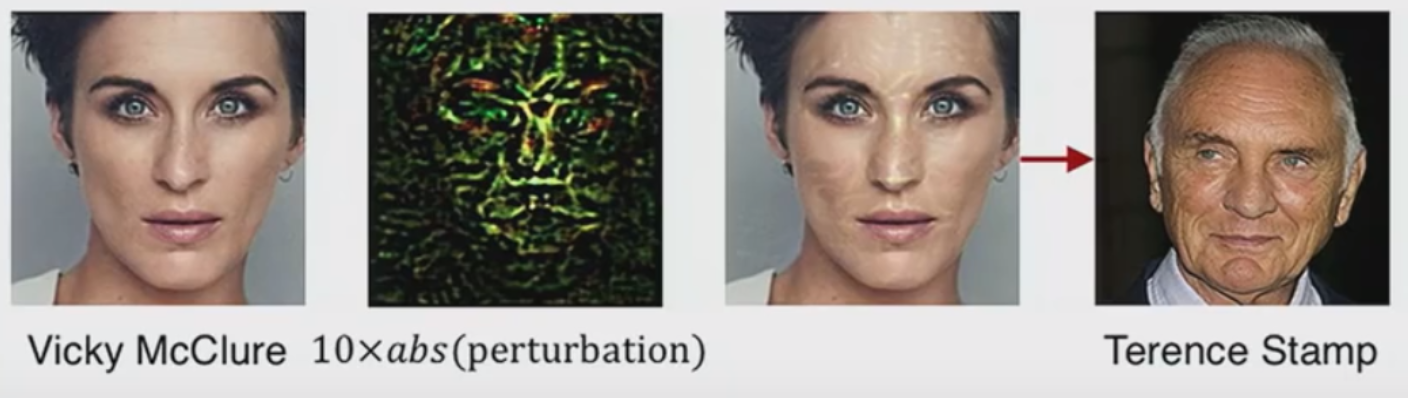
\includegraphics[width=0.8\textwidth]{Images/impersonification.png}
\caption[]{Actress Vicky McClure recognized as Terence Stamp by adding noise to her face image\footnotemark}
\end{figure}

\footnotetext{Image from authors presentation at CCS 2016 \url{https://youtu.be/6Xh1vuwnVhU}}

\subsection{Dodging}

In dogging attacks, an attacker tries to make his / her face misidentified as another face. Attacker don't care as whom  he/she will be classified, the only concern is not to be classified as himself/herself. This can be particularly useful for democratic activists and freedom fighters who live in authoritarian and non-democratic countries. Such activists can use this type of attack to avoid persecution by oppressive governments. From a technical point of view, this category of attack is interesting because causing misclassification should (theoretically) be easier to do with minimal face modifications, compared to incorrectly classifying a face as the specific target (impersonation)